\subsection{Aerodynamics equations for the ailerons}

Now for the ailerons I choose an aileron of the NACA-0009 at 9\% fill which is
used for most control surfaces of this size because it grants a sufficient lift
coefficient as well as a good linear lift region. It grants about 14 to 16
degrees before our aileron stalls. We assume that this is with a relatively
high number of Reynolds which we have a chord of 9 cm. We can see this thanks
to this equation :

\begin{gather*}
    R_e = \frac{\rho V c}{\mu}
\end{gather*}

with $c$ the chord lenght and $V$ the airflow on the ailerons.

So, with our rocket going at max at $130 \si{\meter.\per\second}$ and with a
chord length of $9 \si{\centi\meter}$ we have $36.5 \times 10^5 Re$ which is
considered high ($10^5 to 10^6 Re$ is considered high in aviation) we can also
calculate that our ailerons would have a flow separation between each side of
the ailerons at approximately $10 \si{\degree}$ to $12 \si{\degree}$ of angle
of attack (AoA) which would render our control of the flow non-linear. So, with
this in mind we can limit our AoA at 10° at most in the embedded code as well
as in the simulation.

Now to be able to simulate those ailerons we need to be able to calculate the
torque generated by each aileron to add into the equation of rotation we saw
just above. For each aileron we can determine their impact on the total torque
generated with :

\begin{align*}
    F_L  & = \frac{1}{2} \rho V^2 S C_L (\delta)                    \\
    \tau & = r * F_L                                                \\
         & = r ( \frac{1}{2} \rho V^2 S C_{L \delta} \times \delta) \\
\end{align*}

We can say that :

\begin{gather*}
    K_\tau = \frac{1}{2} \rho V^2 S C_{L \delta} r
\end{gather*}

And thus:

\begin{gather*}
    \tau = K_\tau \times \delta
\end{gather*}

With $V$ the velocity, $S$ the surface $C_{L \delta}$ the derivative of the
lift coefficient, $F_L$ the lift force, $\tau$ the torque, $K_\tau$ the control
effectiveness coefficient, $\delta$ the AoA and r the moment arm which is the
distance between the $CL$ and the $CM$ of the rocket.

To integrate those equations into the simulation we only must determine the
angles of our ailerons over time and input it in the previous equations :

\begin{gather*}
    \tau_i = \frac{1}{2} \rho V^2 S C_{L \delta} r \times \delta_i
\end{gather*}

Our $\delta_i$ will be computed through the output of our simulated PID which
we will see just below this.

With this we can now create our own simulation. We just need to add a few
gaussian noise generators to our system to test our resistance to noise, a
thrust curve to input our thruster in there and a delay between the controller
and the actuators to test even further our model. Which can resemble this:

\begin{figure}[!hbt]
    \centering
    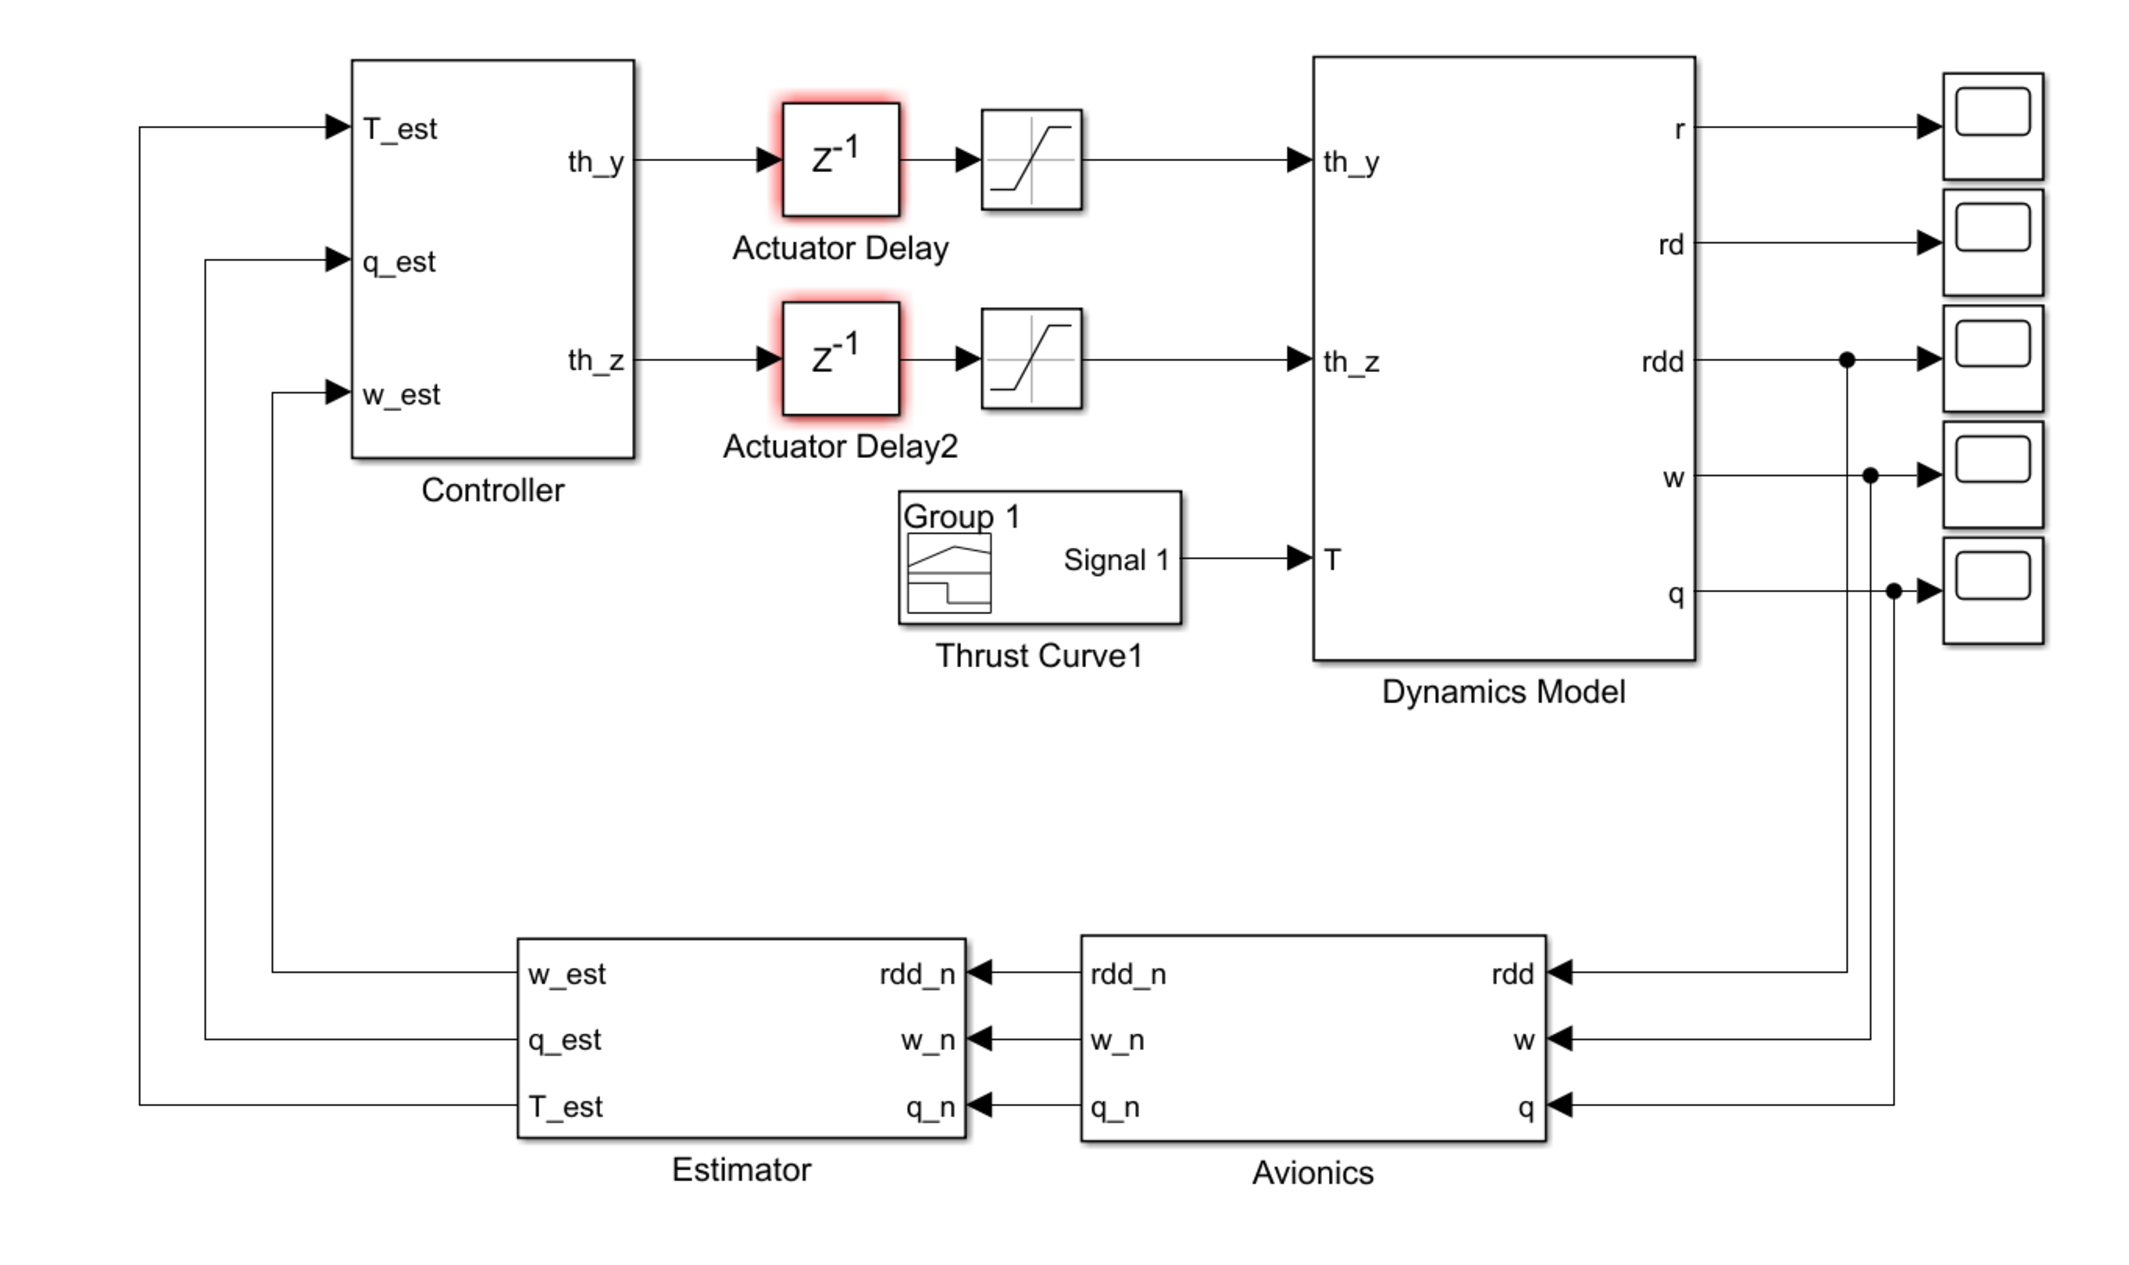
\includegraphics[width=\SchematicWidth]{\Images/rocket_sim/simulink.eps}
    \caption{Simulink model we used}
\end{figure}
\FloatBarrier

To complete our simulation and to be able to compute the angles of every
aileron we need to have some sort of controller. In our case, we will use a PID
controller as it is the controller I am most comfortable with and the one I
understand the most. We create in fact 3 different PID for each axis:

\begin{gather*}
    \delta_{CMD}(t) = K_p e(t) + K_d \frac{de(t)}{dt} + K_i \int e(t) dt
\end{gather*}

After combining each PID we have :

\begin{gather*}
    \overrightarrow{\delta} = M_{control} *
    \begin{bmatrix}
        \delta_P \\
        \delta_Y \\
        \delta_R
    \end{bmatrix}
\end{gather*}

With which we can determine a control matrix to find the effect of each aileron
on a specific axis for example what we have as a control matrix is :

\begin{gather*}
    M_{control} =
    \begin{bmatrix}
        +1 & +1 & +1 \\
        +1 & -1 & -1 \\
        -1 & -1 & +1 \\
        -1 & +1 & -1 \\
    \end{bmatrix}
\end{gather*}

This matrix controls which ailerons move in which direction.